\documentclass[aspectratio=169]{beamer}
\usepackage{graphicx} % Required for inserting images

% \usepackage{armtex}
\usepackage{amsmath}
\usepackage{amsthm}
\usepackage{tikz}
% \usepackage{xcolor}

% \usepackage[usenames,dvipsnames]{xcolor}
\usepackage{algorithm}
\usepackage{algpseudocode}
\usepackage{array}
\usepackage{longtable}
\usepackage{booktabs}
\makeatletter
\def\thmhead@plain#1#2#3{%
  \thmname{#1}\thmnumber{\@ifnotempty{#1}{ }\@upn{#2}}%
  \thmnote{ {\the\thm@notefont#3}}}
\let\thmhead\thmhead@plain
\makeatother

\newcommand{\red}[1]{\textcolor{red}{#1}}
\newcommand{\blue}[1]{\textcolor{blue}{#1}}
\newcommand{\yellow}[1]{\textcolor{yellow}{#1}}
\newcommand{\violet}[1]{\textcolor{violet}{#1}}
\newcommand{\orange}[1]{\textcolor{orange}{#1}}
\newcommand{\green}[1]{\textcolor{green}{#1}}

% ----------------------------\

\usepackage{amsmath}
% \beamertemplatenavigationsymbolsempty

\usetheme{Malmoe}

%gets rid of bottom navigation bars
\setbeamertemplate{footline}[frame number]{}

% %gets rid of bottom navigation symbols
\setbeamertemplate{navigation symbols}{}

%gets rid of footer
%will override 'frame number' instruction above
%comment out to revert to previous/default definitions
\setbeamertemplate{footline}{}

\title{Improving the DSGD Classifier with an Initialization Technique for Mass Assignment Functions}
\author{Tarkhanyan, A. and Harutyunyan, A.}
\date{\today}

\begin{document}

\begin{frame}
  \titlepage
\end{frame}

\begin{frame}
{\small\tableofcontents}
\end{frame}

% \begin{frame}{Նշում}
%     Դիպլոմայինը անգելերով է, սլայդերի մեջ որոշ մասեր նույնպես անգլերենով եմ թողել։ \\ \\ Հույս ունեմ խնդիր չի դա, եթե պետք է արագ կշտկեմ։ \\ \\Շնորհակալություն։    
% \end{frame}

% \section{Հիմնական խնդիրը}
% \subsection{Ձևակերպումը}
% \begin{frame}{Մեկնաբանելիության դերը մեքենայական ուսուցման(ՄՈւ) մեջ}
% \begin{columns}
%   \begin{column}{0.5\textwidth}
%     \begin{itemize}
%       \item Հաճախ բարձր ճշտությամբ մոդելների մոտ առկա է լինում վատ բացատրելի լինելու խնդիրը։
%       \pause
%       \item Բացատրելի մոդել ունենալու խնդիրը երբեմն կրիտիկական կարևորություն է ունենում, օրինակի համար եթե ՄՈւ ալգորիթմի շնորհիվ կայացնենք մարդուն վարկ տալ/չտալու որոշումը ապա որոշ երկրներում օրենքով պարտադրված ենք լինելու նաև այդ մարդուն մերժելու դեպքում տալ համապատասխան հիմնավորումը։
%     \end{itemize}
%   \end{column}
%   \pause
%   \begin{column}{0.5\textwidth}
%     % \includegraphics[width=\textwidth]{"interp_over_power.jpg"}
%     % \pause
%     % \includegraphics[width=\textwidth]{"interp_over_power_accent.jpg"}
%     \begin{overprint}
%         \onslide<3>\includegraphics[width=\textwidth]{"interp_over_power.jpg"}
%         \onslide<4>\includegraphics[width=\textwidth]{"interp_over_power_accent.jpg"}
%     \end{overprint}
% \end{column}  
% \end{columns}
% \end{frame}

% \begin{frame}{Մեկնաբանելիություն ապահովող ալգորիթմներ}
% Կա երկու մոտեցում։
% \begin{itemize}
%     \item Արդեն ունենալով մոդելի կանխագուշակությունները փորձել բացատրել մոդելի աշխատանքը։ \pause
%         \begin{itemize}
%             \item \rm{LIME} (Local Interpretable Model-agnostic Explanations)
%             \item SHAP (SHapley Additive exPlanations)
%         \end{itemize}
%     \pause
%     \item Իսկզբանե բացատրելիությունը ներկառուցել մոդելի մեջ 
%     \begin{itemize}
%         \item Գծային ռեգրեսիա
%         \item Մեր մոտեցումը (Դեմստեր-Շաֆերի տեսություն)
%     \end{itemize}
% \end{itemize}
% \end{frame}


% % \subsection{{\rm LIME (Local Interpretable Model-agnostic Explanations)}}
% % \begin{frame}{{\rm LIME (Local Interpretable Model-agnostic Explanations)}}
% %   \begin{itemize}
% %     \item \textbf{Նպատակը:} Բացատրել կանխագուշակությունները ամեն կետի համար որոշակի լոկալ տիրույթում կլասիֆիկացիայի բացատրելի ալգորիթմ կիրառելով։ \pause
% %     \item \textbf{Քայլերը:} 
% %       \begin{enumerate} 
% %         \item Գեներացնել կետեր տրված կետի որոշակի շրջակայքում և օգտագործել տրամադրած մոդելը պիտակներ ստանալու համար։ 
% %         \item Կշիռ տալ այդ գեներացված կետերին ըստ նրանց և սկզբնական կետի Էվկլիդյան հեռավորության
% %         \item Աշխատացնել բացատրելի մոդել (օրինակ գծային ռեգրեսիա), որը ստանալով այդ գեներացված կետերը կկանխագուշակի տրամադրած մոդելի պիտակները։
% %       \end{enumerate}
% %     \end{itemize}
% % \end{frame}

% % \begin{frame}{Մաթեմատիկական ձևակերպումը։}
% %     \textbf{Մաթեմատիկական ձևակերպումը}
% %     \begin{itemize}
% %         \item Դիցուք \( x \)-ը կետ է որի համար պետք ա ստանանք մեկնաբանությունները և \( \xi \)-ն որևէ բացատրելի մոդել է (օրինակ գծային ռեգրեսիա).
% %         \item Գեներացնել նոր կետերի \( Z \) բազմությունը \( \mathcal{N}(x, \sigma^2) \) բաշխումից որտեղ \( \sigma \)-ն կառավարում է թե որքան լոկալ ենք ուզում լինեն մեր բացատրությունները.
% %         \item Լոկալ \( \xi \) մոդելին սովորացնում ենք մինիմիզացնել
% %           \[
% %           \mathcal{L}(f, \xi, \pi_x) = \sum_{z, z' \in Z} \pi_x(z) \left(f(z) - \xi(z')\right)^2
% %           \]
% %            ֆունկցիան որտեղ \( \pi_x(z) \) կշիռները սահմանող ֆունկրան է, \( f \)-ը մեզ տրամադրված մոդելը, իսկ \( Z \)-ը գեներացված կետերի բազմությունն է.
% %     \end{itemize}
% %     \textbf{Մեկնաբանումը:} \( \xi \) մոդելի գործակիցները իրենցից ներկայացնելու ենք \( x \) կետի վրա տարբեր ատրիբուտների ազդեցությունները։
% % \end{frame}

\begin{frame}
    \begin{center}
        \Huge Dempster-Shafer theory
    \end{center}
\end{frame}

\section{Dempster-Shafer theory (DST)}
\begin{frame}{Dempster-Shafer theory (DST)}
    \begin{block}{ԴՍՏ-ի ընդհանուր նկարագիրը}
        DST (also known as "theory of belief functions") provides a
mathematical approach for combining evidence from different sources to calculate
the probability of an event, utilizing Dempster’s rule of combination. 
            % \vspace{0.5cm}
            % \\
        % \pause
        % Հիմնական կարևորությունը կայանում է պատահույթների {\rm "plausability"}-ն գնահատելու մեջ։     \vspace{0.5cm}
        % \pause
        % ԴՍՏ-ն կարող ենք դիտարկել որպես Բայեսի տեսության ընդհանրացում։
        
    \end{block}
\end{frame}


% \subsection{{\rm Mass Assignment} ֆունկցիաներ}
% \begin{frame}{{\rm Mass Assignment Function (MAF)}}
%   \begin{itemize}
%     \item \textbf{Մաթեմատիկական ձևակերպումը:}
%       \begin{itemize}
%         \item Դիցուք \( X \)-ը պատահույթների բազմությունն է, որը հայտնի է որպես {\rm frame of discernment} \pause
%         \item {\rm Mass assignment function} \( m \)-ը ֆունկցիա է որոշված $X$-ի ենթաբազմությունների բազմության՝ \( 2^X \) վրա այնպես որ՝
%           \[
%           m : 2^X \rightarrow [0, 1]
%           \]
%         \pause
%         \item Տեղի ունեն հետևյալ պայմանները։
%           \begin{enumerate}
%             \item \( m(\emptyset) = 0 \) (Դատարկ բազմությունը կշիռ չունի)
%             \item \( \sum\limits_{A \subseteq X} m(A) = 1 \) (Կշիռների գումարը միշտ 1 է)
%           \end{enumerate}
%       \end{itemize}
%   \end{itemize}
% \end{frame}

% \begin{frame}{{\rm MAF}-ի օրինակներ}
% \begin{itemize}
%     \item Պատկերացնենք որ ազնիվ կոպեկ ենք նետում, կլասիկ հավանականային մոդելի դեպքում սա կարող ենք արտահայտել որպես $P(\{heads\}) = (\{tails\}) = 0.5$, ԴՍՏ մոդելի դեպքում էլ կլինի $P(\varepsilon) = 0, P(\{heads\}) = (\{tails\}) = 0.5, P(\{heads, tails\}) = 0$:
%     \pause
%     \item Իսկ եթե կոպեկը անարդար լիներ կլասիկ մոտեցմանբ ոչմի բան չէինք կարող պնդել, մինչդեռ ԴՍՏ-ով կարող ենք ասել որ $P(\varepsilon) = 0, P(\{heads\}) = (\{tails\}) = 0, P(\{heads, tails\}) = 1$:
%     \pause
%     \item Օրինակ որտեղ կարող է շողալ ԴՍՏ-ն հետևայլն է։ Պատկերացնենք ինչ-որ մարդ իր կողքով անցնող մեքենա է տեսել և անում է հետևյալ պնդումը։ 
%     \begin{enumerate}
%         \item Մեքենայան կամ սև էր կամ շականակագույն, ամեն դեպքում ոնց-որ թե սև էր, բայց դե գուցե սխալվում եմ։ 
%         Այս դեպքում {\rm MAF}—ը կարող է ունենալ այսպիսի տեսք։ $m(\{\varnothing\}) = 0.1, m(\{ black\}) = 0.4, m(\{ brown\}) = 0.3, m(\{ black, brown\} = 0.2$
%     \end{enumerate}
%     % same as prob. dist. func
% \end{itemize}
% \end{frame}

% \subsection{{\rm Belief} և {\rm Plausibility}}
% \begin{frame}{{\rm Belief} և {\rm Plausibility}}
%     \begin{block}
%          $\forall  A  \in X $
%           \[
%           Bel(A) = \sum_{B \subseteq A} m(B)
%           \]
%         \[
%           Pl(A) = \sum_{B \cap A \neq \emptyset} m(B)
%           \]
%             \[
%             Bel(A) \le P(A) \le Pl(A)
%             \]

%     Նախորդ օրինակի դեպքում սև մեքենայի համար կունենանք՝
%     $m(\{\varnothing\}) = 0.1, m(\{ black\}) = 0.4, m(\{ brown\}) = 0.3, m(\{ black, brown\} = 0.2$ \\
%     $A$ = սև, $B$ = շակագույն
%           \[
%         Bel(A) = m(A) = 0.4 \]
%         \[
%         Pl(A) = m(A) + m(\{A, B\}) = 0.4 + 0.2 = 0.6
%           \]
%     \end{block}
%     % \begin{block}
    
%     % \end{block}
% \end{frame}

% % ԹՈՒԴՈՒ
% \subsection{Դեմստերի օրենք}
% \begin{frame}{Դեմստերի օրենք}
% \begin{itemize}
%   \item Դեմստերի օրենքը կիրառվում է \(m_1\) և \(m_2\) {\rm MAF}-ը միավորելու համար.
%   \item \textbf{Բանաձևը}
%     \begin{equation*}
%       m_f(A) = m_1(A) \oplus m_2(A) = \frac{1}{1 - K} \sum_{B \cap C = A} m_1(B) m_2(C)
%     \end{equation*}
%     \pause
%   \item \textbf{Անհամաձայնության չափ \(K\):}
%     \begin{equation*}
%       K = \sum_{B \cap C = \emptyset} m_1(B) m_2(C)
%     \end{equation*}
%     \pause
%   \item Եթե $K=1$ հանգում ենք զրոյի բաժանման խնդրի։
%   \end{itemize}
% \end{frame}

% \begin{frame}{}
%     \begin{block}{Աբելյան կիսախումբ}
% \begin{itemize}
%   \item Դիցուք \(M_{\Omega}\)-ն բոլոր հնարավոր {\rm MAF}-երի բազմությունն է սահմանված \(\Omega\) պատահույթների բազմության վրա: \pause
%   \item \((M_{\Omega}, \oplus)\)-ն հանդիսանում է Աբելյան կիսախումբ: 
%   \begin{itemize}
%     \item Ասոցատիվություն \( m_1 \oplus (m_2 \oplus m_3) = (m_1 \oplus m_2) \oplus m_3 \)
%     \item Կոմուտատիվություն \( m_1 \oplus m_2 = m_2 \oplus m_1 \)
%   \end{itemize}
% \end{itemize}
% \end{block}
% \pause
% \begin{block}{Զրոյացնող ({\rm Absorbent}) և միավոր էլեմենտ}
% \begin{itemize}
%   \item Կլանող էլեմենտ
%   \begin{itemize}
%     \item Դիցուք \(C_A : 2^X \to [0, 1]\) այնպես որ \(C_A(A) = 1\) և \(\forall Y \neq A, C_A(Y) = 0\).
%     \item Ապա \(m \oplus C_A = C_A\).
% \pause
%   \end{itemize}
%   \item Միավոր էլեմենտ:
%   \begin{itemize}
%     \item Դիցուք \(U : 2^X \to [0, 1]\) այնպես որ \(U(X) = 1\) և \(\forall Y \neq X, U(Y) = 0\).
%     \item Ապա \(m \oplus U = m\).
%   \end{itemize}
% \end{itemize}
% \end{block}

% \end{frame}


\section{Old Approach}

\begin{frame}
    \begin{center}
        \Huge Old approach
    \end{center}
\end{frame}

\begin{frame}{Old approach}
    In order to get the prediction
\begin{enumerate}
    \item For the given dataset $RS$ rule set is generated.
    \item Each rule's corresponding $MAF$ gets initiated in the following way:: Uncertainty (whole set) gets 0.8 weight, and the remaining 0.2 weight is randomly split between $singletron$ elements.
    \item For given input $x$:
\end{enumerate}

\end{frame}

\begin{frame}
\begin{figure}
    \centering
    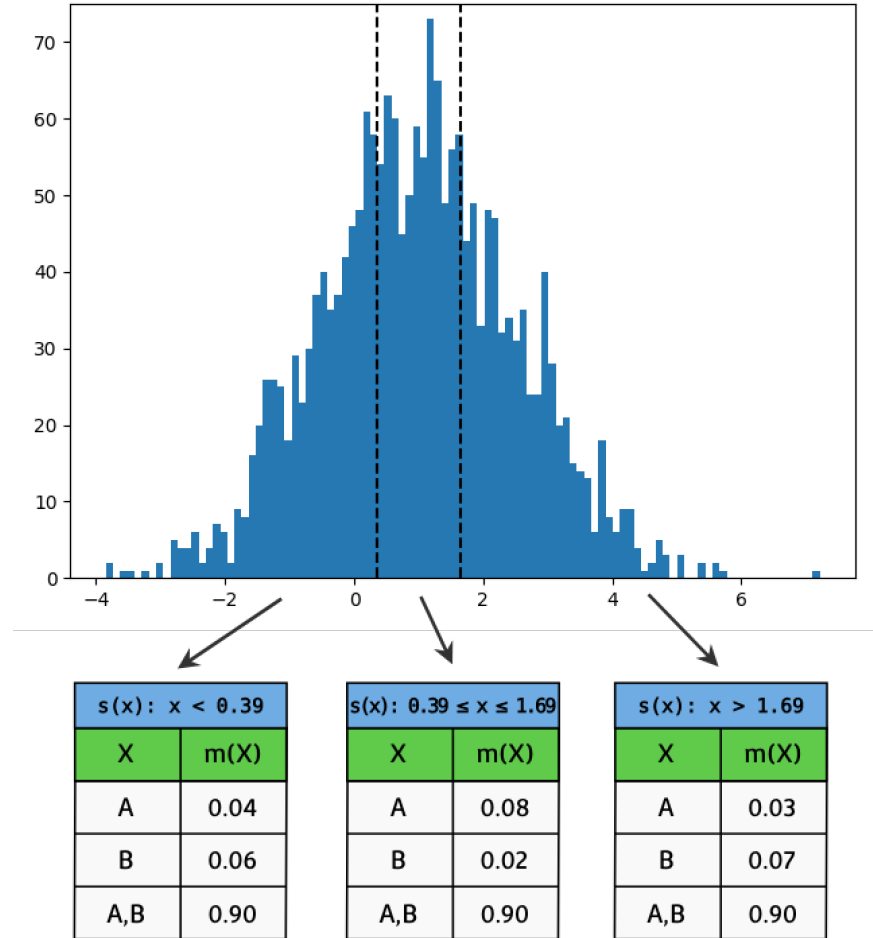
\includegraphics[width=0.45\linewidth]{image.png}
    \label{fig:enter-label}
\end{figure}
    
\end{frame}



\begin{frame}{Old approach}
\begin{align*}
\mathcal{M}_x &= \left\{ m \mid (m, s) \in RS \land x \right\} \\
m_f &= \bigoplus_{m \in \mathcal{M}_x} m \\
\hat{y} &= \underset{{\rm class}}{\mathrm{argmax}} \, {\rm Bel}(m_f)
\end{align*}

\end{frame}

% \begin{frame}{Օպտիմիզացիա}
%     Օգտագործում ենք $ADAM$ ալգորիթմը։
% \begin{align*}
% m_t &= \beta_1 m_{t-1} + (1 - \beta_1) \frac{dJ}{d\theta} \\
% v_t &= \beta_2 v_{t-1} + (1 - \beta_2) \left(\frac{dJ}{d\theta}\right)^2 \\
% \hat{m}_{t+1} &= \frac{m_t}{1 - \beta_1^t} \\
% \hat{g}_{t+1} &= \frac{v_t}{1 - \beta_2^t} \\
% \theta_{t+1} &= \theta_t - \frac{\alpha \hat{m}_{t+1}}{\sqrt{\hat{g}_{t+1}} + \varepsilon}
% \end{align*}
% \end{frame}

% where: TODO
% \begin{itemize}
%   \item \( m_t \) and \( v_t \) are estimates of the first moment (the mean) and the second moment (the uncentered variance) of the gradients, respectively.
%   \item \( \frac{dJ}{d\theta} \) is the gradient of the objective function \( J \) with respect to the parameters \( \theta \) for the current time step.
%   \item \( \beta_1 \) and \( \beta_2 \) are the exponential decay rates for the moment estimates.
%   \item \( \hat{m}_t \) and \( \hat{v}_t \) are bias-corrected versions of \( m_t \) and \( v_t \).
%   \item \( \alpha \) is the step size.
%   \item \( \epsilon \) is a small scalar used to prevent division by zero.
%   \item \( \theta_t \) are the parameters to be updated.
% \end{itemize}

\begin{frame}{Loss function}
    \begin{block}{Mean squared error}
        \begin{equation}
MSE = \frac{1}{n} \sum_{i=1}^{n} \left\| y_i - \hat{y}_i \right\|^2
        \end{equation}
    \end{block}
    \begin{block}{{\rm Cross-Entropy}}
        \begin{equation}
        CE = - \frac{1}{n} \sum_{i=1}^{n} \sum_{j=1}^{k} y_{ij} \cdot \log(\hat{y}_{ij})
        \end{equation}
    
    \end{block}
        
\end{frame}
\begin{figure}
    \centering
    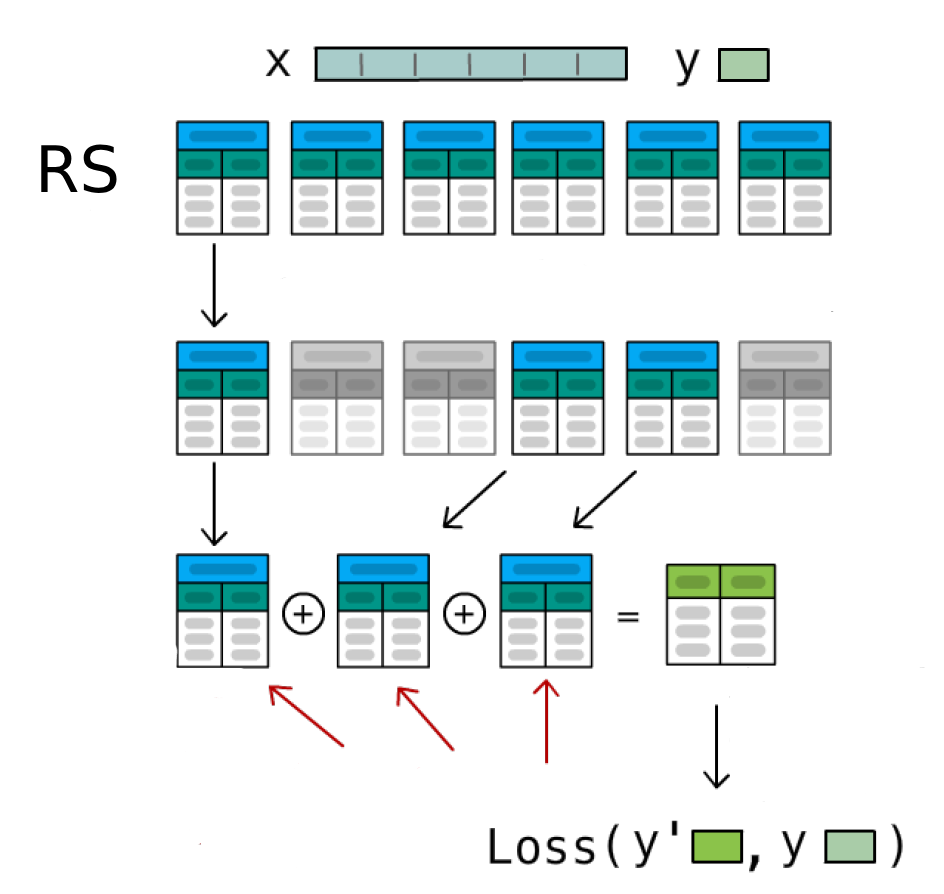
\includegraphics[width=0.55\linewidth]{dst_ill_eng.png}
\end{figure}




\section{Our approach}
\begin{frame}
    \begin{center}
        \Huge Our approach
    \end{center}
\end{frame}
\subsection{{\rm KMeans}}
\begin{frame}
\begin{figure}
    \centering
    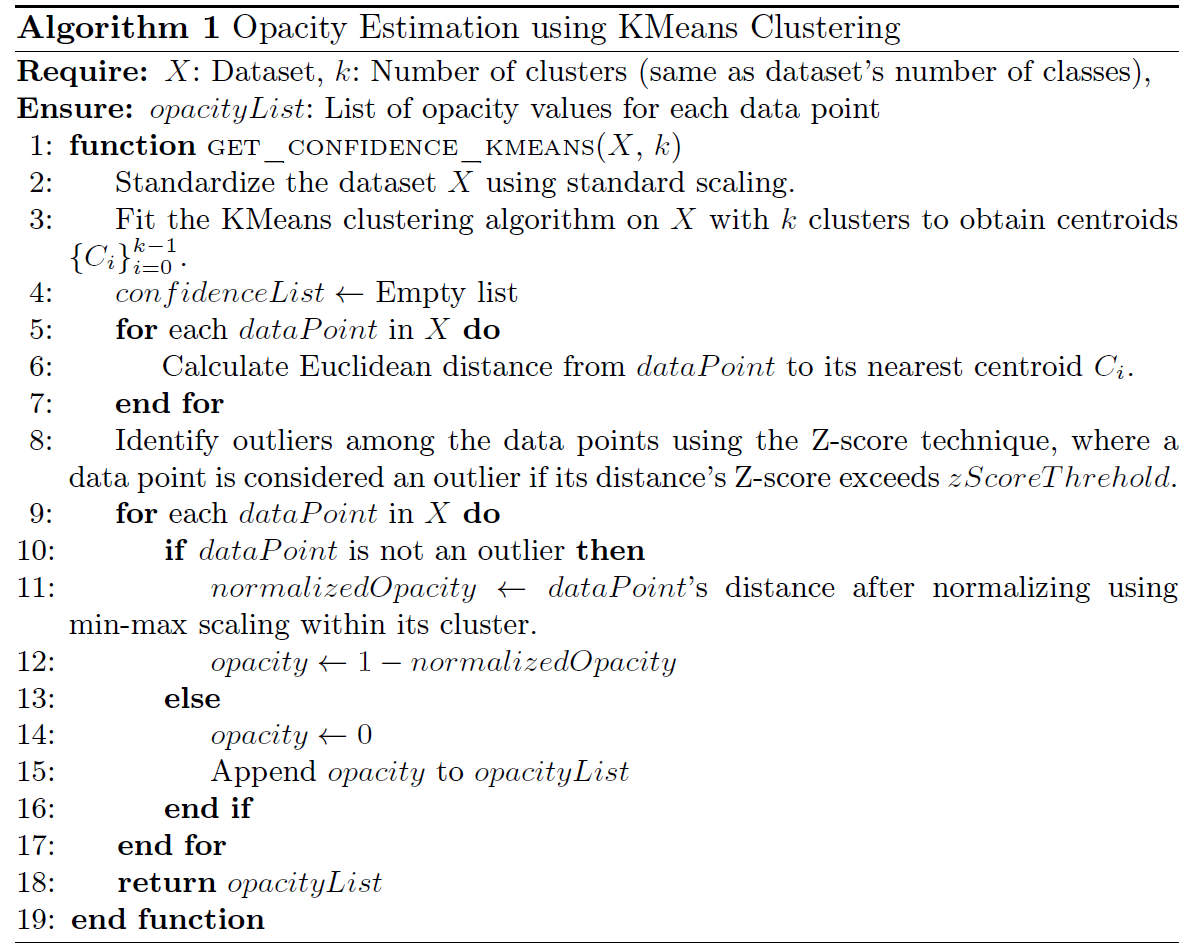
\includegraphics[width=0.68\linewidth]{alg_kmeans_opacity.png}
    \caption{Enter Caption}
    \label{fig:enter-label}
\end{figure}
\end{frame}

% BRING BACK TODO
\begin{frame}
\begin{figure}
    \centering
    \includegraphics[width=0.78\linewidth]{kmeans_opactiy.png}
    \label{fig:enter-label}
\end{figure}
\end{frame}

\subsection{{\rm DBSCAN}}
\begin{frame}
\begin{figure}
    \centering
    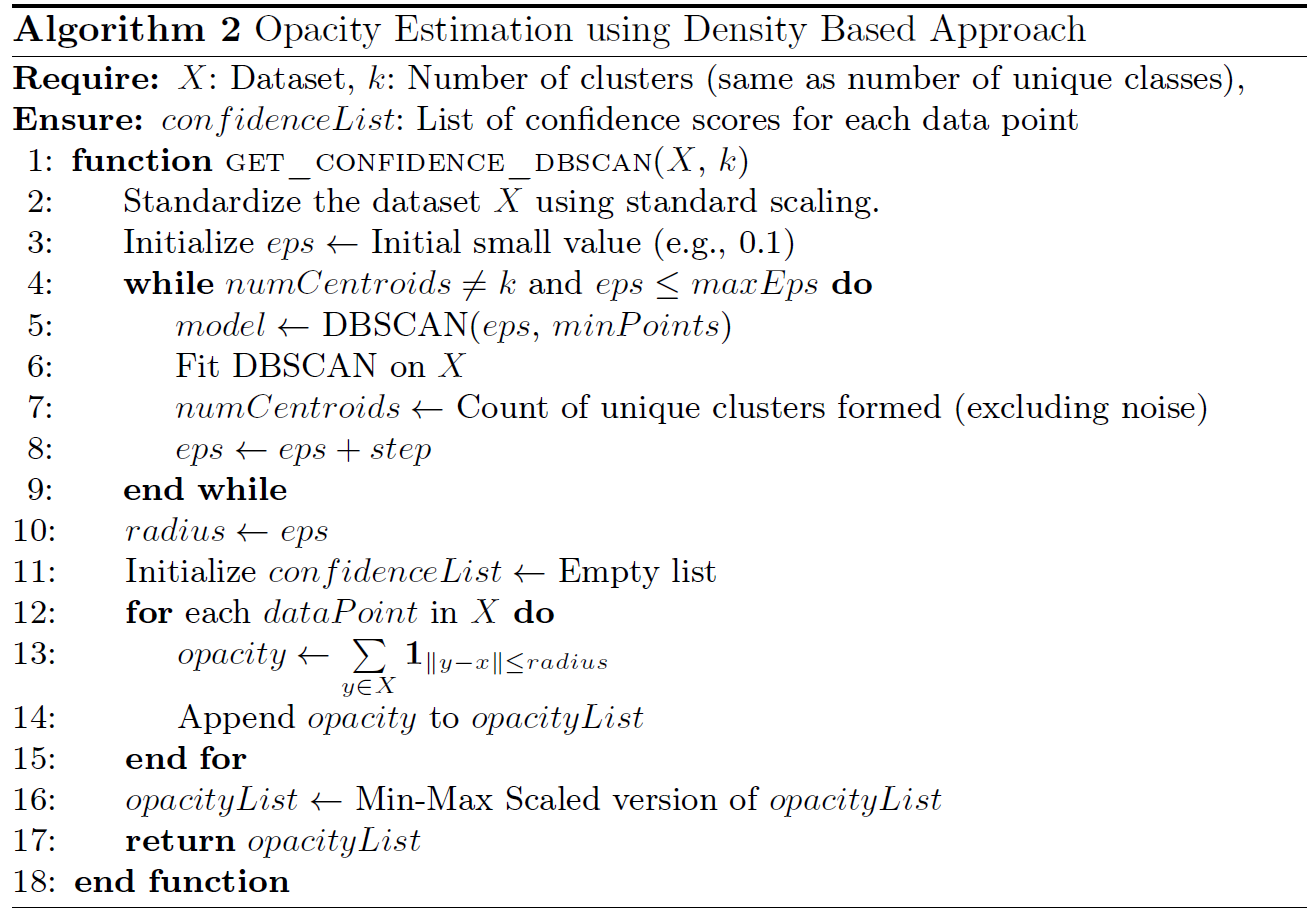
\includegraphics[width=0.75\linewidth]{alg_dbscan_opacity.png}
    \label{fig:enter-label}
\end{figure}
    
\end{frame}


\begin{frame}
\begin{figure}
    \centering
    \includegraphics[width=0.75\linewidth]{denisty_opactiy.png}
    \label{fig:enter-label}
\end{figure}
\end{frame}

\subsection{Rule confidence estimation}
\begin{frame}{Rule Confidenceի գնահատում}

\begin{enumerate}
    \item Filter the dataset to retain only the rows that comply with the rule. \pause
    \item If the rule does not apply to any rows, set its confidence to 0 (this corresponds
to the full uncertainty). Otherwise: \pause
    \item Calculate the rule’s confidence as the mean representativeness of the rows it
covers. \pause
    \item If the rows are not homogeneous with respect to their labels, reduce the
confidence based on the proportion of the most frequent label among these
rows.
\end{enumerate} 
\end{frame}


% \subsection{{\rm MAF}-ի ինիցալիզացիա}
% \begin{frame}{{\rm MAF Initialization}}
% \begin{block}
%     {\rm
%     In the Mass Assignment Function (MAF), we use the following values for initialization. Let $c = get\_confidence(rule)$ represent the confidence derived for a given rule. The label $l_{\text{mode}}$, which is the most frequently occurring label within the subset of data points covered by the rule, receives the confidence value $c$. The remaining mass, $(1 - c)$, is evenly distributed among all other labels present in the subset. Formally, for an element $l_i$ in the subset:
% \[
% m(l_i) = 
% \begin{cases} 
% c & \text{if } l_i = l_{\text{mode}}, \\
% \frac{1-c}{n-1} & \text{otherwise},
% \end{cases}
% \]
% where $m(l_i)$ denotes the mass assigned to label $l_i$, and $n$ is the total number of elements in the frame of discernment. 
% }
% \end{block}

% \end{frame}

\subsection{MAF Initialization}
\begin{frame}{MAF Initialization}
\[
m(l_i) = 
\begin{cases} 
c & \text{if } l_i = l_{\text{{\rm mode}}}, \\
\frac{1-c}{n-1} & \text{otherwise},
\end{cases}
\]


\end{frame}




\section{Results}


\begin{frame}
    \begin{center}
        \Huge Data
    \end{center}
\end{frame}

\subsection{{Data}}
\begin{frame}{Data}
{\rm
\begin{longtable}{|>{\raggedright\arraybackslash}p{3cm}|c|c|>{\raggedright\arraybackslash}p{5cm}|}
\hline
\textbf{Dataset} & \textbf{Rows} & \textbf{Columns} & \textbf{Description} \\ \hline
\endfirsthead
\hline
\textbf{Dataset} & \textbf{Rows} & \textbf{Columns} & \textbf{Description} \\ \hline
\endhead
Brain Tumor & 3762 & 14 & Includes first-order and texture features with target levels. \\ \hline
Breast Cancer Wisconsin & 699 & 9 & Clinical reports detailing cell benignity or malignancy. \\ \hline
Gaussian & 500 & 3 & Two 2D Gaussian distributions generate this dataset. \\ \hline
Uniform & 500 & 3 & Uniform samples from [-5, 5], with class split by the sign of x. \\ \hline
Rectangle & 1263 & 3 & Points in [-1, 1]×[-1, 1], class determined by the y component's sign. \\ \hline
\end{longtable}
    }
\end{frame}

\subsection{Accuracy and Speedup Analysis}
\begin{frame}{Accuracy and Speedup Analysis}
\begin{figure}
    \centering
    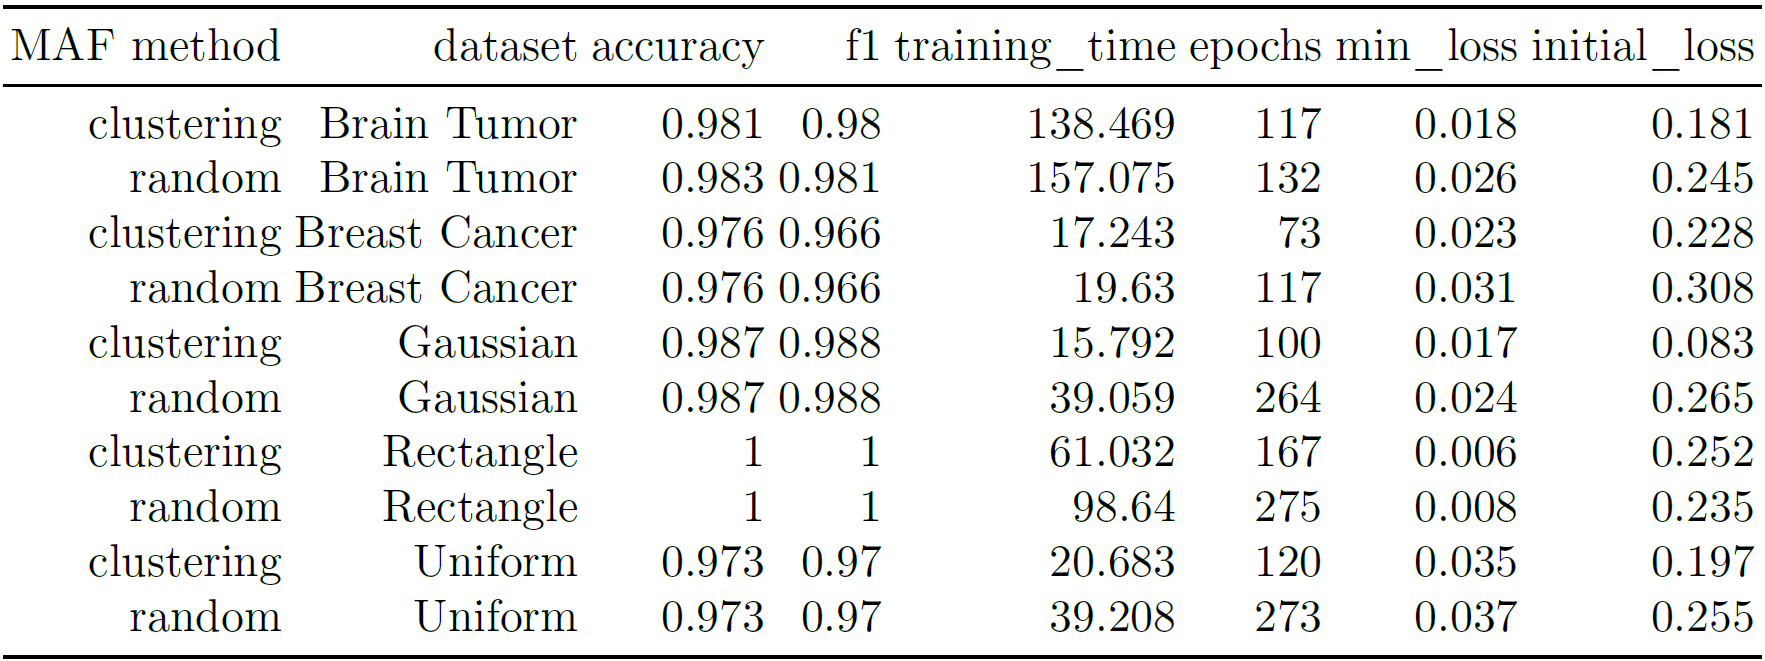
\includegraphics[width=0.95\linewidth]{acc_speedup_table.png}
    % \caption{Enter Caption}
    \label{fig:enter-label}
\end{figure}
\end{frame}

\begin{frame}
\begin{figure}
    \centering
    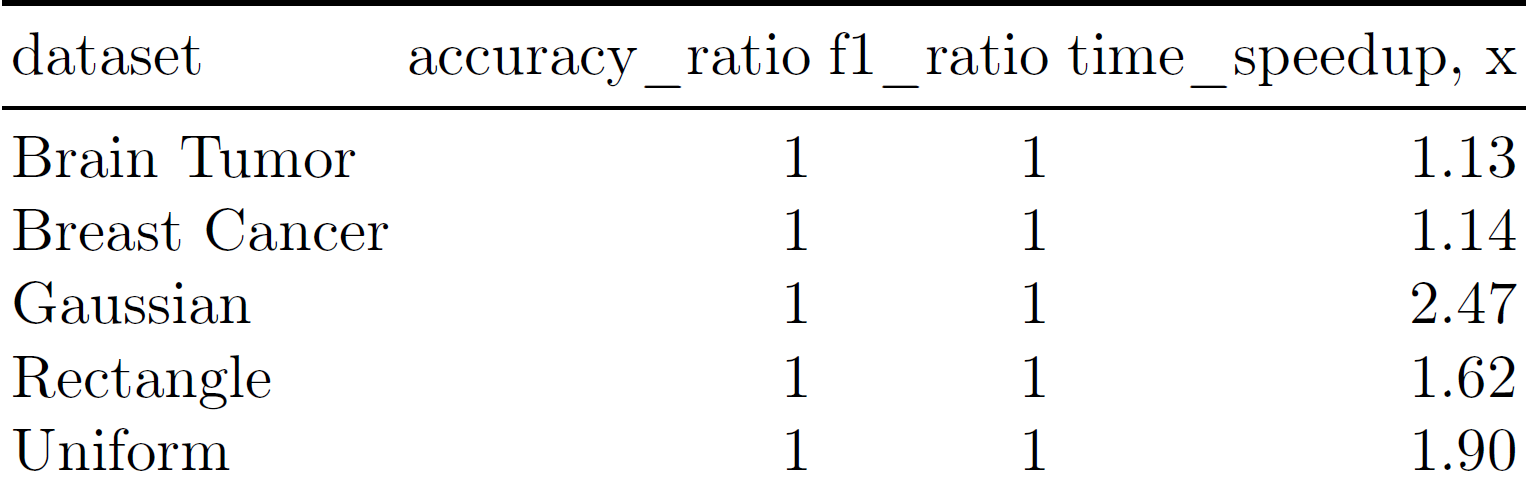
\includegraphics[width=1\linewidth]{speedup_groupby.png}
\end{figure}
\textbf{Average speedup - 1.65{\rm x}}
    
\end{frame}

\begin{frame}
    \begin{figure}
    \centering
    \begin{minipage}{0.49\textwidth}
        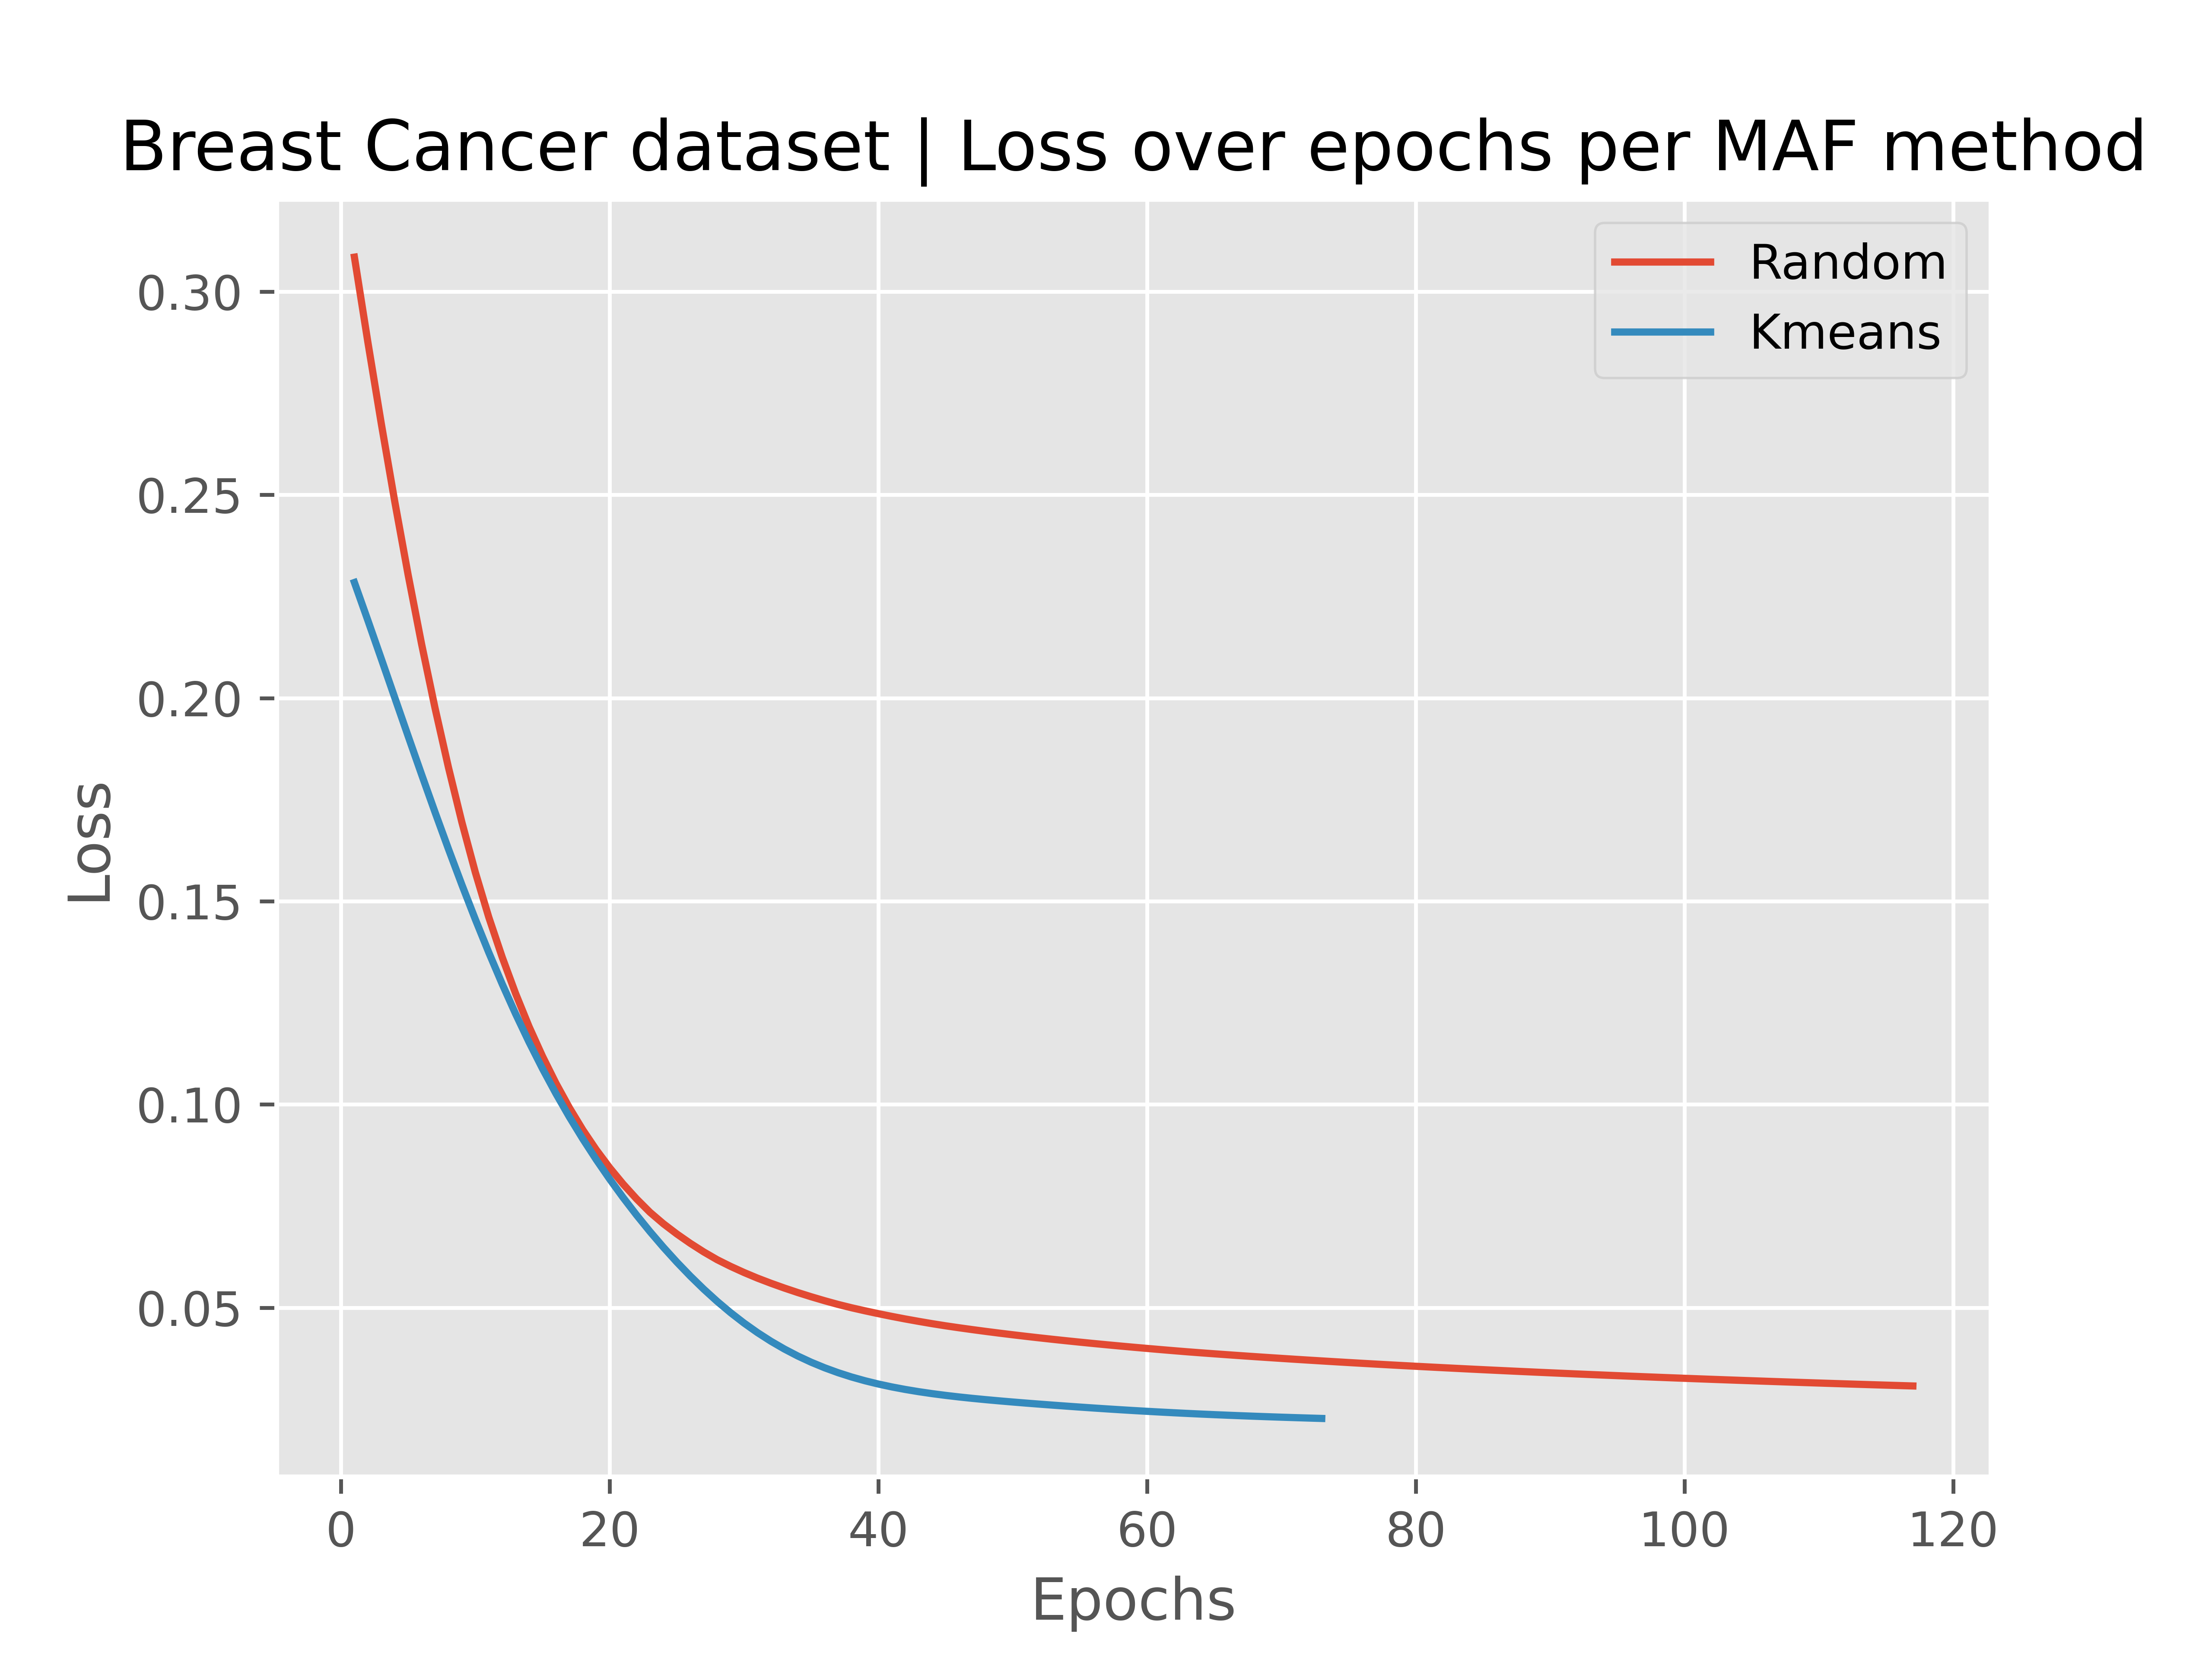
\includegraphics[width=\linewidth]{breast-cancer-wisconsin_loss.png} % First image
    \end{minipage}\hfill
    \begin{minipage}{0.49\textwidth}
        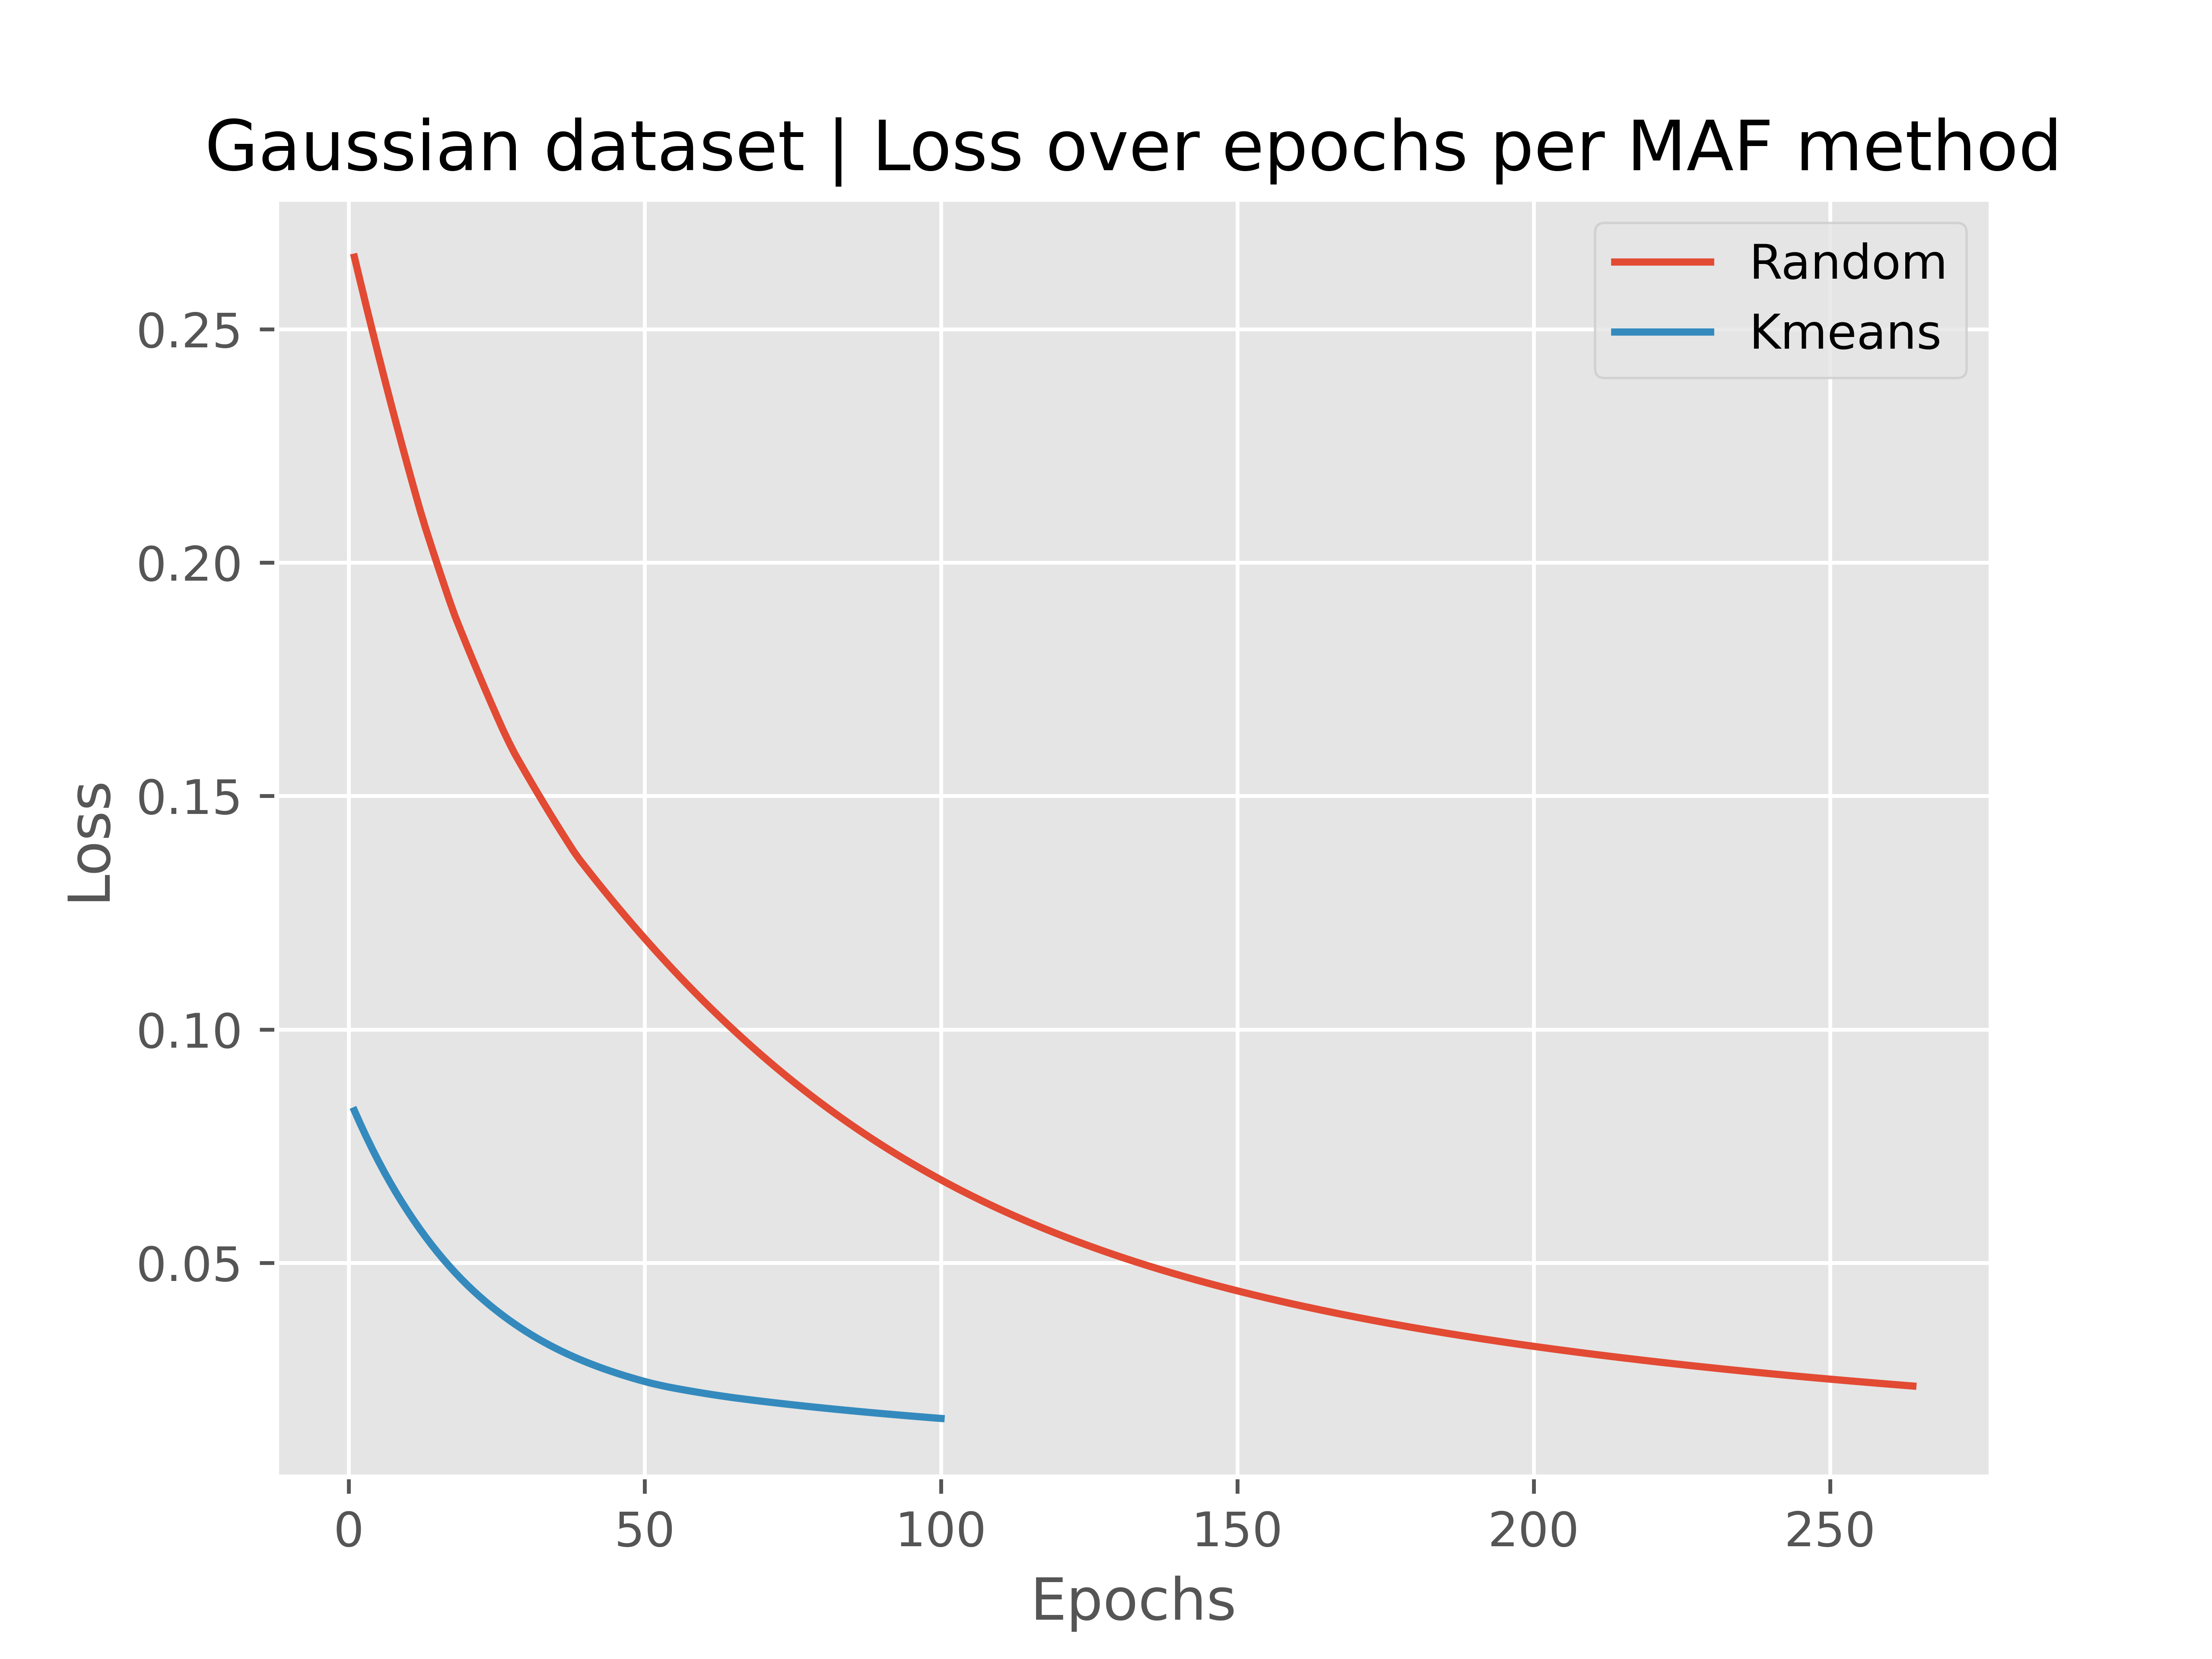
\includegraphics[width=\linewidth]{gaussian_df_loss.png} % Second image
    \end{minipage}
    \caption{The figure demonstrates the benefits offered by MAF initialization, mainly
decreased number of epochs and better starting point.}
    \label{fig:side_by_side}
\end{figure}
\end{frame}

\subsection{Uncertainty Analysis}
\begin{frame}{{\rm Pitfall of the current approach}}
\begin{figure}
    \centering
    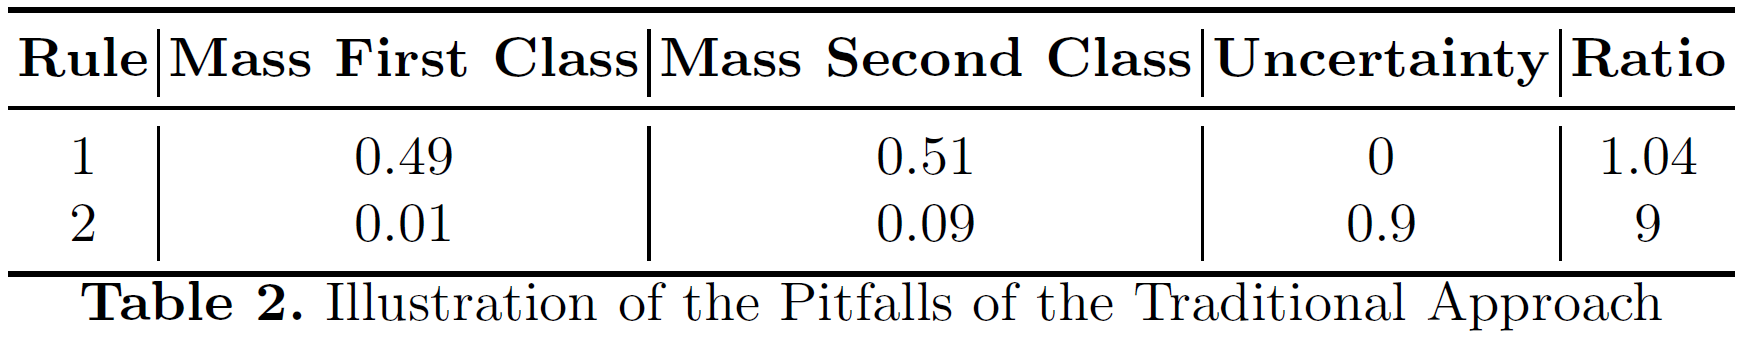
\includegraphics[width=1\linewidth]{pitfalls.png}
\end{figure}
\end{frame}

\begin{frame}
\begin{itemize}
\item \textbf{Uncertainty Adjustment:}
    \[
    U' = 1 - U
    \]
    where \( U \) is the original uncertainty.
    \pause
    \item \textbf{Normalization of the Ratio:}
    \[
    R' = \frac{R - \min(R)}{\max(R) - \min(R)}
    \]
    where \( R \) is the original ratio (when dividing the values of two masses we
add $\varepsilon=0.01$ to denominator to avoid zero division error), and \( \min(R) \) and \( \max(R) \) are the minimum and maximum values of the ratio across all rules,
respectively.
    \pause
    \item \textbf{Harmonic Mean Calculation:}
    \[
    H = \frac{2 \cdot U' \cdot R'}{U' + R'}
    \]
     
\end{itemize}
\end{frame}

\begin{frame}
\begin{figure}
    \centering
    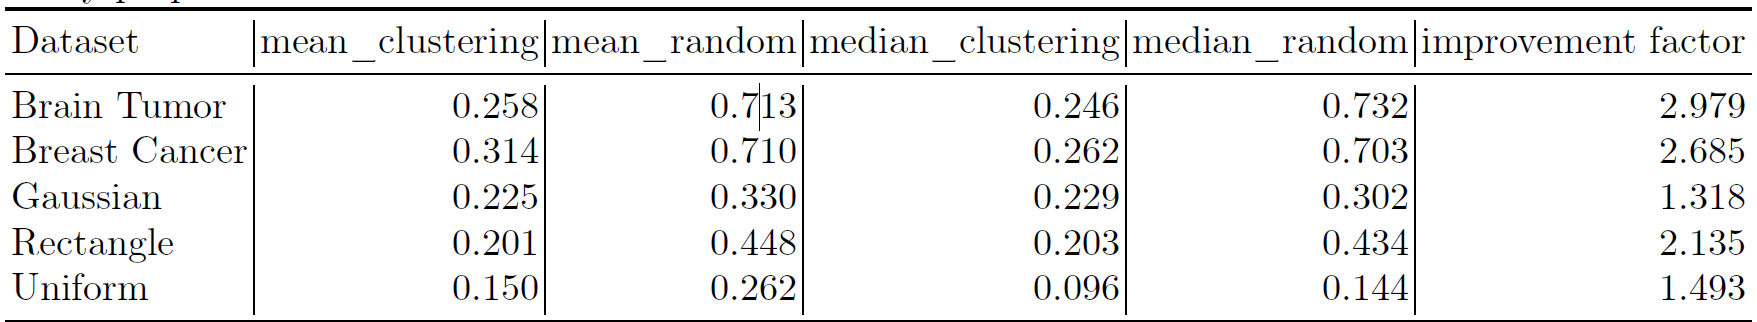
\includegraphics[width=1\linewidth]{unc_df.png}
\end{figure}
{\rm $improvement\_factor$} is defined as the ratio of $median\_random$ and $median\_clustering$. 

On average the clustering approach yields in uncertainty reduction
by a factor of \textbf{2.12}.
    
\end{frame}

\begin{frame}
\begin{figure}
    \centering
    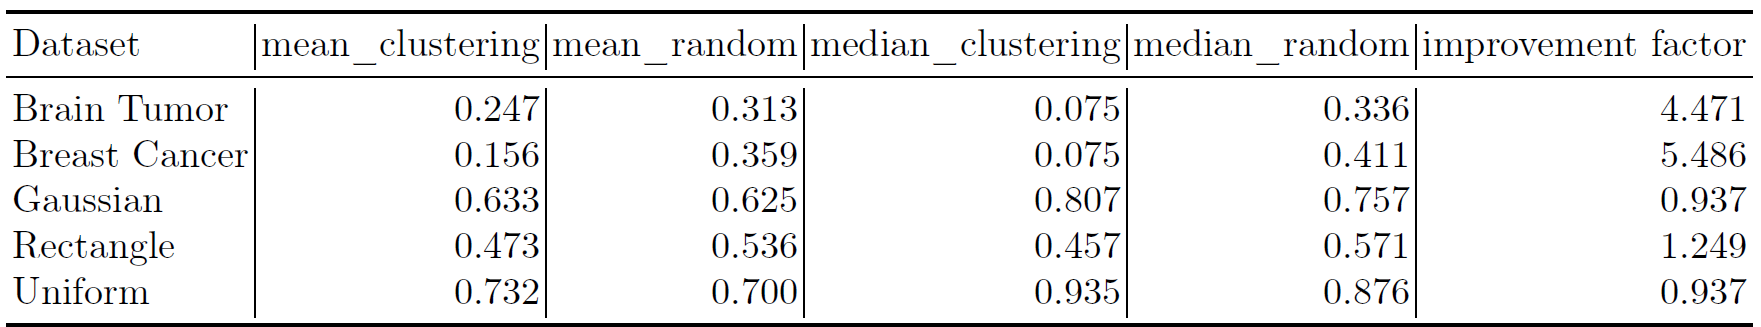
\includegraphics[width=1\linewidth]{score_df.png}
\end{figure}
On average the clustering approach yields in uncertainty
reduction (harmonic mean approach) by a factor of \textbf{2.61}.
\end{frame}

\begin{figure}
\begin{figure}
    \makebox[\textwidth][c]{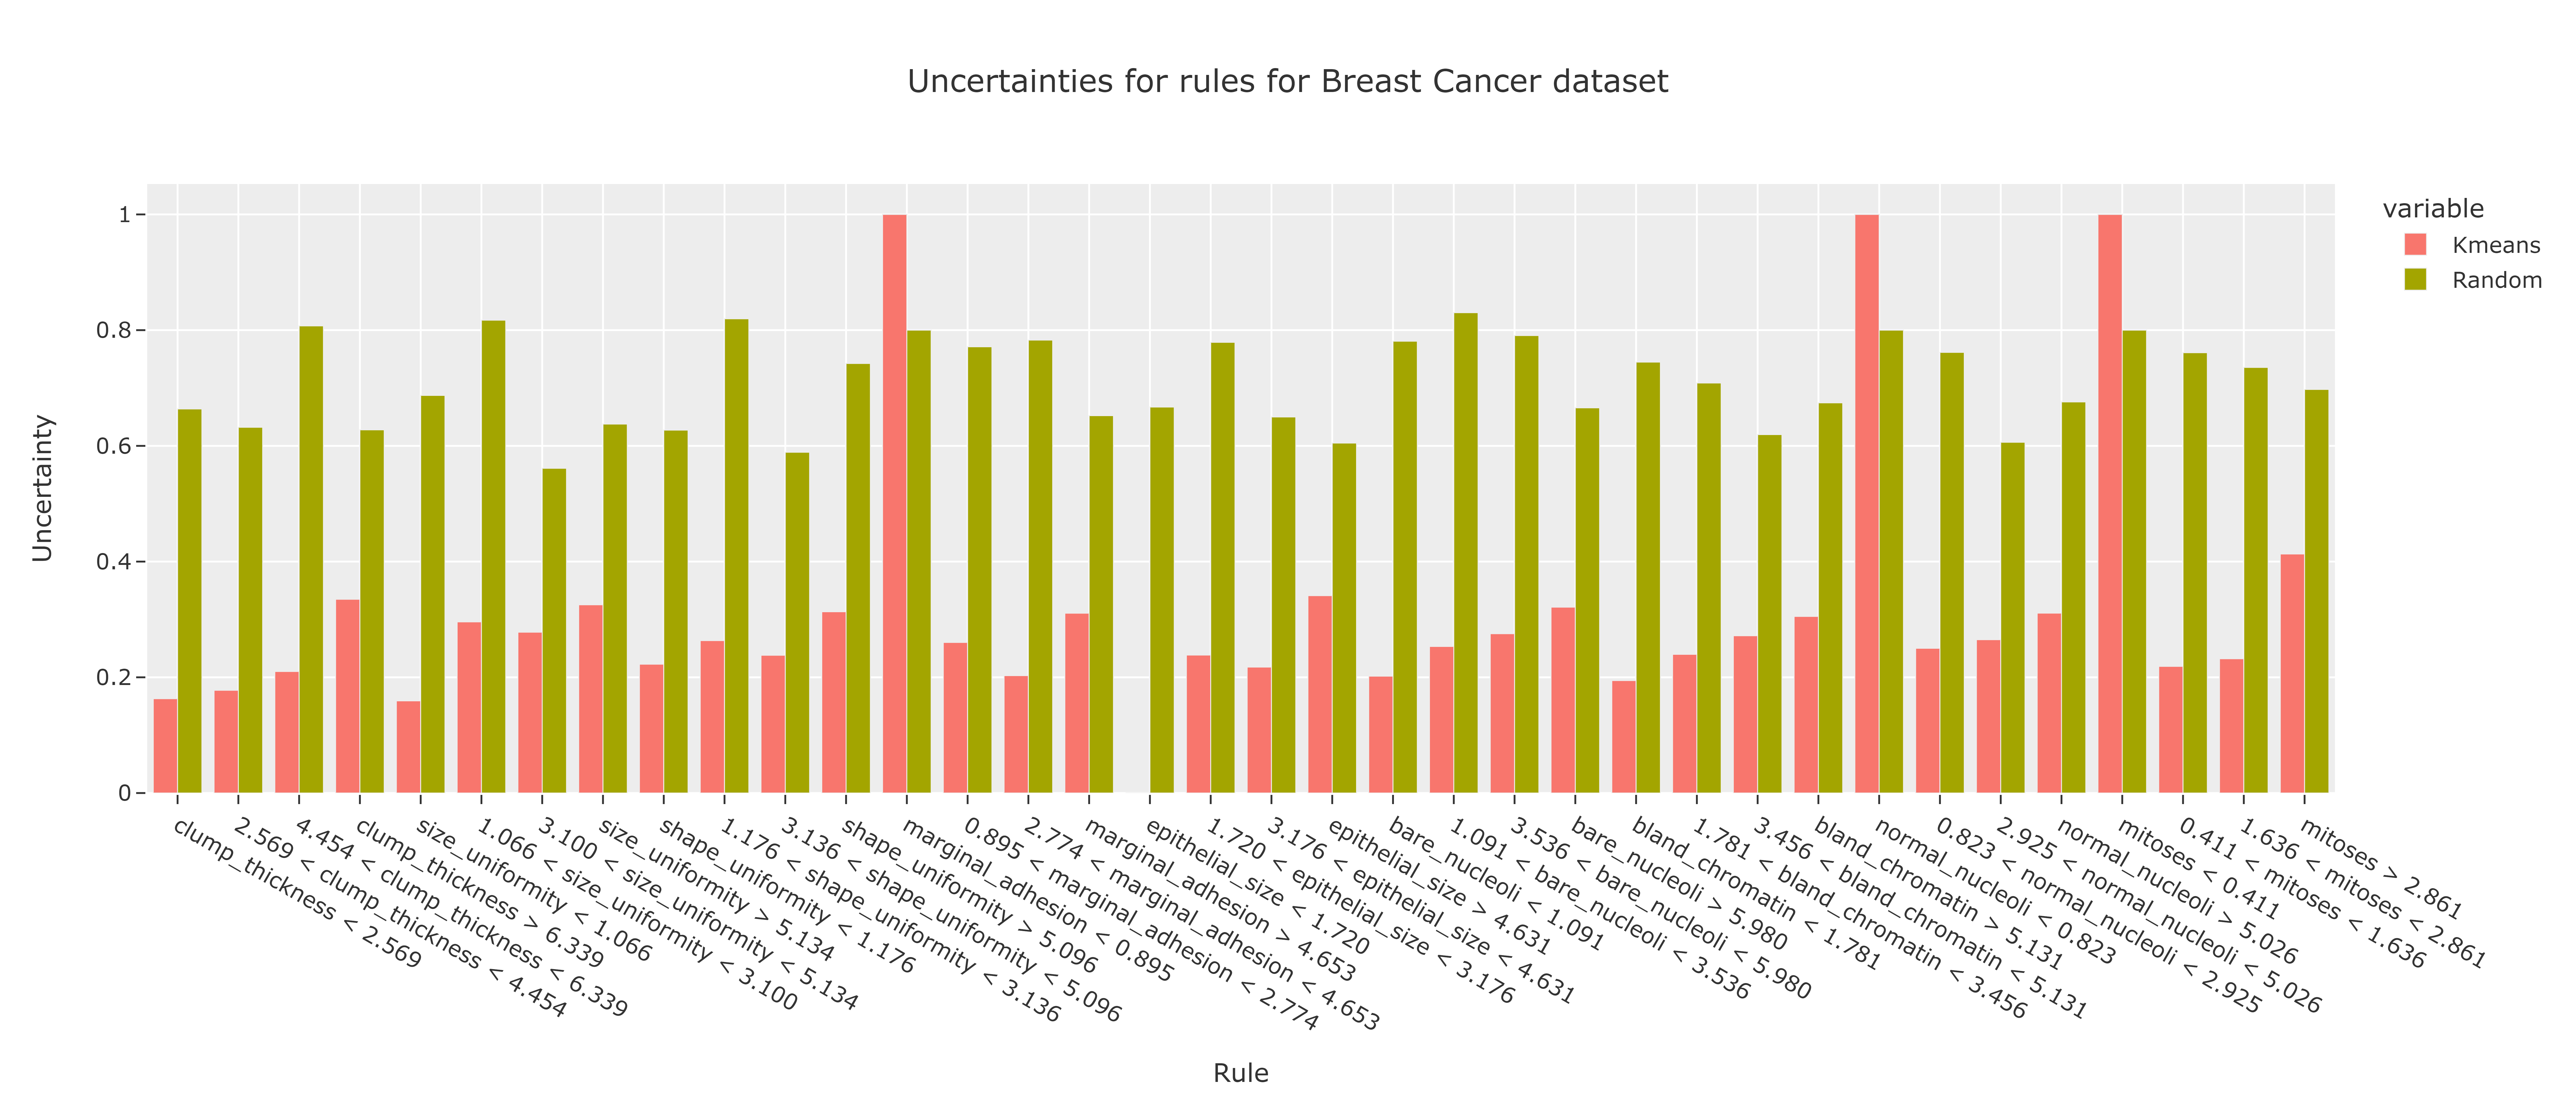
\includegraphics[width=\linewidth]{bars.png}} 
    \caption{Uncertainties per rule for different MAF initialization methods}
    \label{fig:bars}
\end{figure}
\end{figure}

\begin{frame}{Գրականություն}
    
\begin{thebibliography}{8}
{\rm
\bibitem{dst}
Shafer, G.: A Mathematical Theory of Evidence. Princeton University Press, Princeton (1976)

\bibitem{sergio}
Peñafiel, S., Baloian, N., Sanson, H., \& Pino, J. A.: Applying Dempster–Shafer theory for developing a flexible, accurate and interpretable classifier. Expert Systems with Applications \textbf{148}, 113262 (2020)

\bibitem{kmeans}
J. MacQueen . Some methods for classification and analysis of multivariate observations. Proc. Fifth Berkeley Symp. on Math. Statist. and Prob., Vol. 1 (Univ. of Calif. Press, ), 281--297. (1967)

\bibitem{breastCancer}
Wolberg, W. H., Mangasarian, O. L.: Multisurface method of pattern separation for medical diagnosis applied to breast cytology. Proceedings of the National Academy of Sciences \textbf{87}(23), 9193--9196 (1990)

\bibitem{brainTumor}
Bohaju, J.: Brain Tumor. In: Kaggle 2020, DOI: \doi{10.34740/KAGGLE/DSV/1370629}. \url{https://www.kaggle.com/dsv/1370629} (2020)
}
\end{thebibliography}
\end{frame}

% \begin{frame}
% \begin{figure}
%     \centering
%     
\includegraphics[scale=0.27]{AUA_Codassca2024_website-100-2048x596.jpg}
% \end{figure}
    
% \end{frame}

\begin{frame}
    \begin{center}
        \Huge Thank you
    \end{center}
\end{frame}


\end{document}


% ToDO if have time
% \section{SHAP Interpretability}
% \begin{frame}{SHAP Interpretability: A Mathematical View}
%   \begin{itemize}
%     \item \textbf{Objective:} SHAP provides a unified measure of feature importance based on Shapley values from cooperative game theory.
%     \item \textbf{Process:}
%       \begin{enumerate}
%         \item Calculate the contribution of each feature to the prediction by considering all possible combinations of features.
%         \item This involves computing the difference in the model's prediction with and without the feature, averaged over all possible subsets of features.
%       \end{enumerate}
%     \item \textbf{Mathematical Formulation:}
%       \begin{itemize}
%         \item Let \( f \) be the prediction model, \( x \) be the instance to explain, and \( S \subseteq F \setminus \{i\} \) where \( F \) is the set of all features and \( i \) is a feature.
%         \item The SHAP value \( \phi_i \) for feature \( i \) is given by:
%           \[
%           \phi_i(f, x) = \sum_{S \subseteq F \setminus \{i\}} \frac{|S|! (|F| - |S| - 1)!}{|F|!} [f_x(S \cup \{i\}) - f_x(S)]
%           \]
%         \item Here, \( f_x(S) \) is the prediction of model \( f \) with features in set \( S \) active, and the term outside the brackets is a weight representing the number of ways to form \( S \).
%       \end{itemize}
%     \item \textbf{Interpretation:} SHAP values explain the prediction of instance \( x \) by quantifying the contribution of each feature to the difference between the actual prediction and the average prediction.
%   \end{itemize}
% \end{frame}



